% Experiments

\chapter{Experimentation}

In this chapter, we will go through the process, result, and analysis of two experiments for Voxer's comparative testing in Keravan Energy's cooling system. The \gls{cad} models for pipeline is shown in appendix \ref{appx:second}; and source code for analysis are also presented in appendix \ref{appx:first}. Figure \vref{fig:original_pipe} shows the original cooling piping section in Keravan Energy. The pipeline includes these main components: one 5 meters of straight pipe, two $90^{\circ}$ elbows and rubber hoses. The pipe used in Keravan Energy is DN50. In these experiments, the fluid flows were recognized as turbulent flow. Turbulent flow occurs when instabilities in a flow are not sufficiently damped by viscous action and the fluid velocity at each point in the flow exhibits random fluctuations \cite{turbulent:article}. The fluid tested in both of experiment was a Newtonian fluid, water, at moderate temperatures.


\section{Laboratory experimentation}

It is essential to get a full understanding of the hydraulic system, product testing, and objectives. In order to achieve this, it is advised to perform comparative measurements under laboratory condition first. In this setting, we will acquire more knowledge about factors which could affect the system, proper techniques, required conditions and practices which needed to be applied to ensure the quality of the measurement. Moreover, the data acquired would be more stable under a controlled setting.

\subsection{Experiment's design}

The main goal of this laboratory experimentation is setting up the closest replication of cooling piping section with \gls{pp} material and determining which Voxer combination is the best for the real test in Keravan Energy. 
\begin{figure}[h]
  \centering
  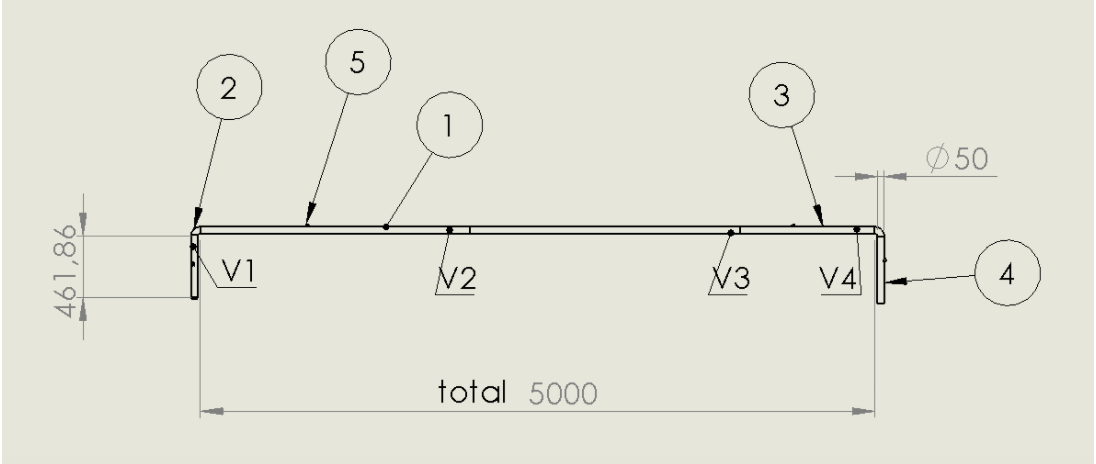
\includegraphics[width=11cm]{cadlab}
  \caption{ Basic pipe layout and positions of measuring points and Voxer wings \newline 1) Straight pipes $2\ m$; 2) $90^{\circ}$ pipe bends; 3) Straight pipe $1\ m$; 4) Straight pipe $0.5\ m$; 5) Plane connectors for measuring points}
  \label{fig:cadlab}
\end{figure}

\gls{cad} drawing in figure \vref{fig:cadlab} illustrates the basic setting of the pipeline. There were 4 measuring points which associated with plane connectors. The reason for creating these connectors is to create the flat surface for ensuring secured pressurization of measuring points. It also minimized the interference of the measuring device to the pressure and flow in the system. Each Voxer was connected to the end of each straight pipe, except the last one. There were maximum 4 Voxers using in each of measurement. With this setting, the pipeline was divided into 3 sections as pipes in series where total pressure is the accumulation of pressure from each section of the whole pipeline. In this experiment, we named section A from point 1 to 2, section B from point 2 to 3 and section C from point 3 to 4. Section T indicates the whole pipe from point 1 to 4 as the beginning and the end of the system. 
Since all of the pipes were connected in series, we have:
\begin{align}
\Delta P_t&= P_a + P_b + P_c = P_ab + P_c 
\end{align}
$\Delta P_t$ is the total pressure change in pipeline; $P_a$, $P_b$ and $P_c$ are the pressure change in section A, B and C; $P_{ab}$ is the pressure change in section A and B together.

There were 2 types of Voxer which were used in the test: Voxer $40^{\circ}$ DN40 and Voxer $30^{\circ}$ DN40. The angle indicates the direction of the outcome flow after going through the Voxer wing. Different combinations of the amount of Voxer and types of Voxer were carried out to determine the behavior of flow in each section and find out the best combination. 
Table \ref{table:combi} lists out the combinations performed in this test. $V1$ was placed before the $1^{st}$ elbow in section A. Section B included $V2$ and $V3$ at the end of each 2-meter-pipe. The last Voxer $V4$ was placed before the ending curved pipe in section C. The mixed combination included $30^{\circ}$ Voxer as $V1$ and $40^{\circ}$ Voxer as $V4$. The pressure changes between section A, section A and B and total pipe were measured in every combination. Every measurement was repeated 10 times to ensure balanced values. During the test, the average temperature of water in the vessel was measured also to consider its influence on fluid \gls{viscos} and surface tension. Measurement for pipe without Voxer installed was performed as well. The inner diameter of the pipe was measured to have Voxer customized as a perfect fit inside the tube. The material of pipes is \gls{pp}. 

\begin{table}[h]
  \centering
  \caption{Voxer combinations in lab test.}
  \begin{tabular}{l*{6}{c}}
Type             & V0 & V1 & V12 & V123 & V1234 & V14 \\
\hline
None & X & - & - & - & - & -   \\
30 degree           & - & X & X & X &  X & X  \\
40 degree           & - & X & X & X &  X & X   \\
Mixed     & - & - & - & - & - & X   \\
\end{tabular}
  \label{table:combi}
\end{table}

\subsection{Setting of experiments}

\textbf{Main pipe} \newline
The tested pipeline system was set like figure \vref{fig:cadlab} in Metropolia’s laboratory.  Pipes were connected with others in series. The main straight horizontal pipe section is $5\ m$ long in total, which included two $2\ m$ of straight pipes and one $1\ m$ of straight pipe. Each side of main straight pipe was fitted with a $90^{\circ}$ curved pipe. There were two $0.5\ m$ of vertical pipe extensions at each side, acting as extended pipes for placing Voxer and measuring points. Two reducers were attached with these extended in order to accommodate the hose pump. Figure \vref{fig:wholepipe} demonstrates the completed setting.

\begin{figure}[h]
  \centering
  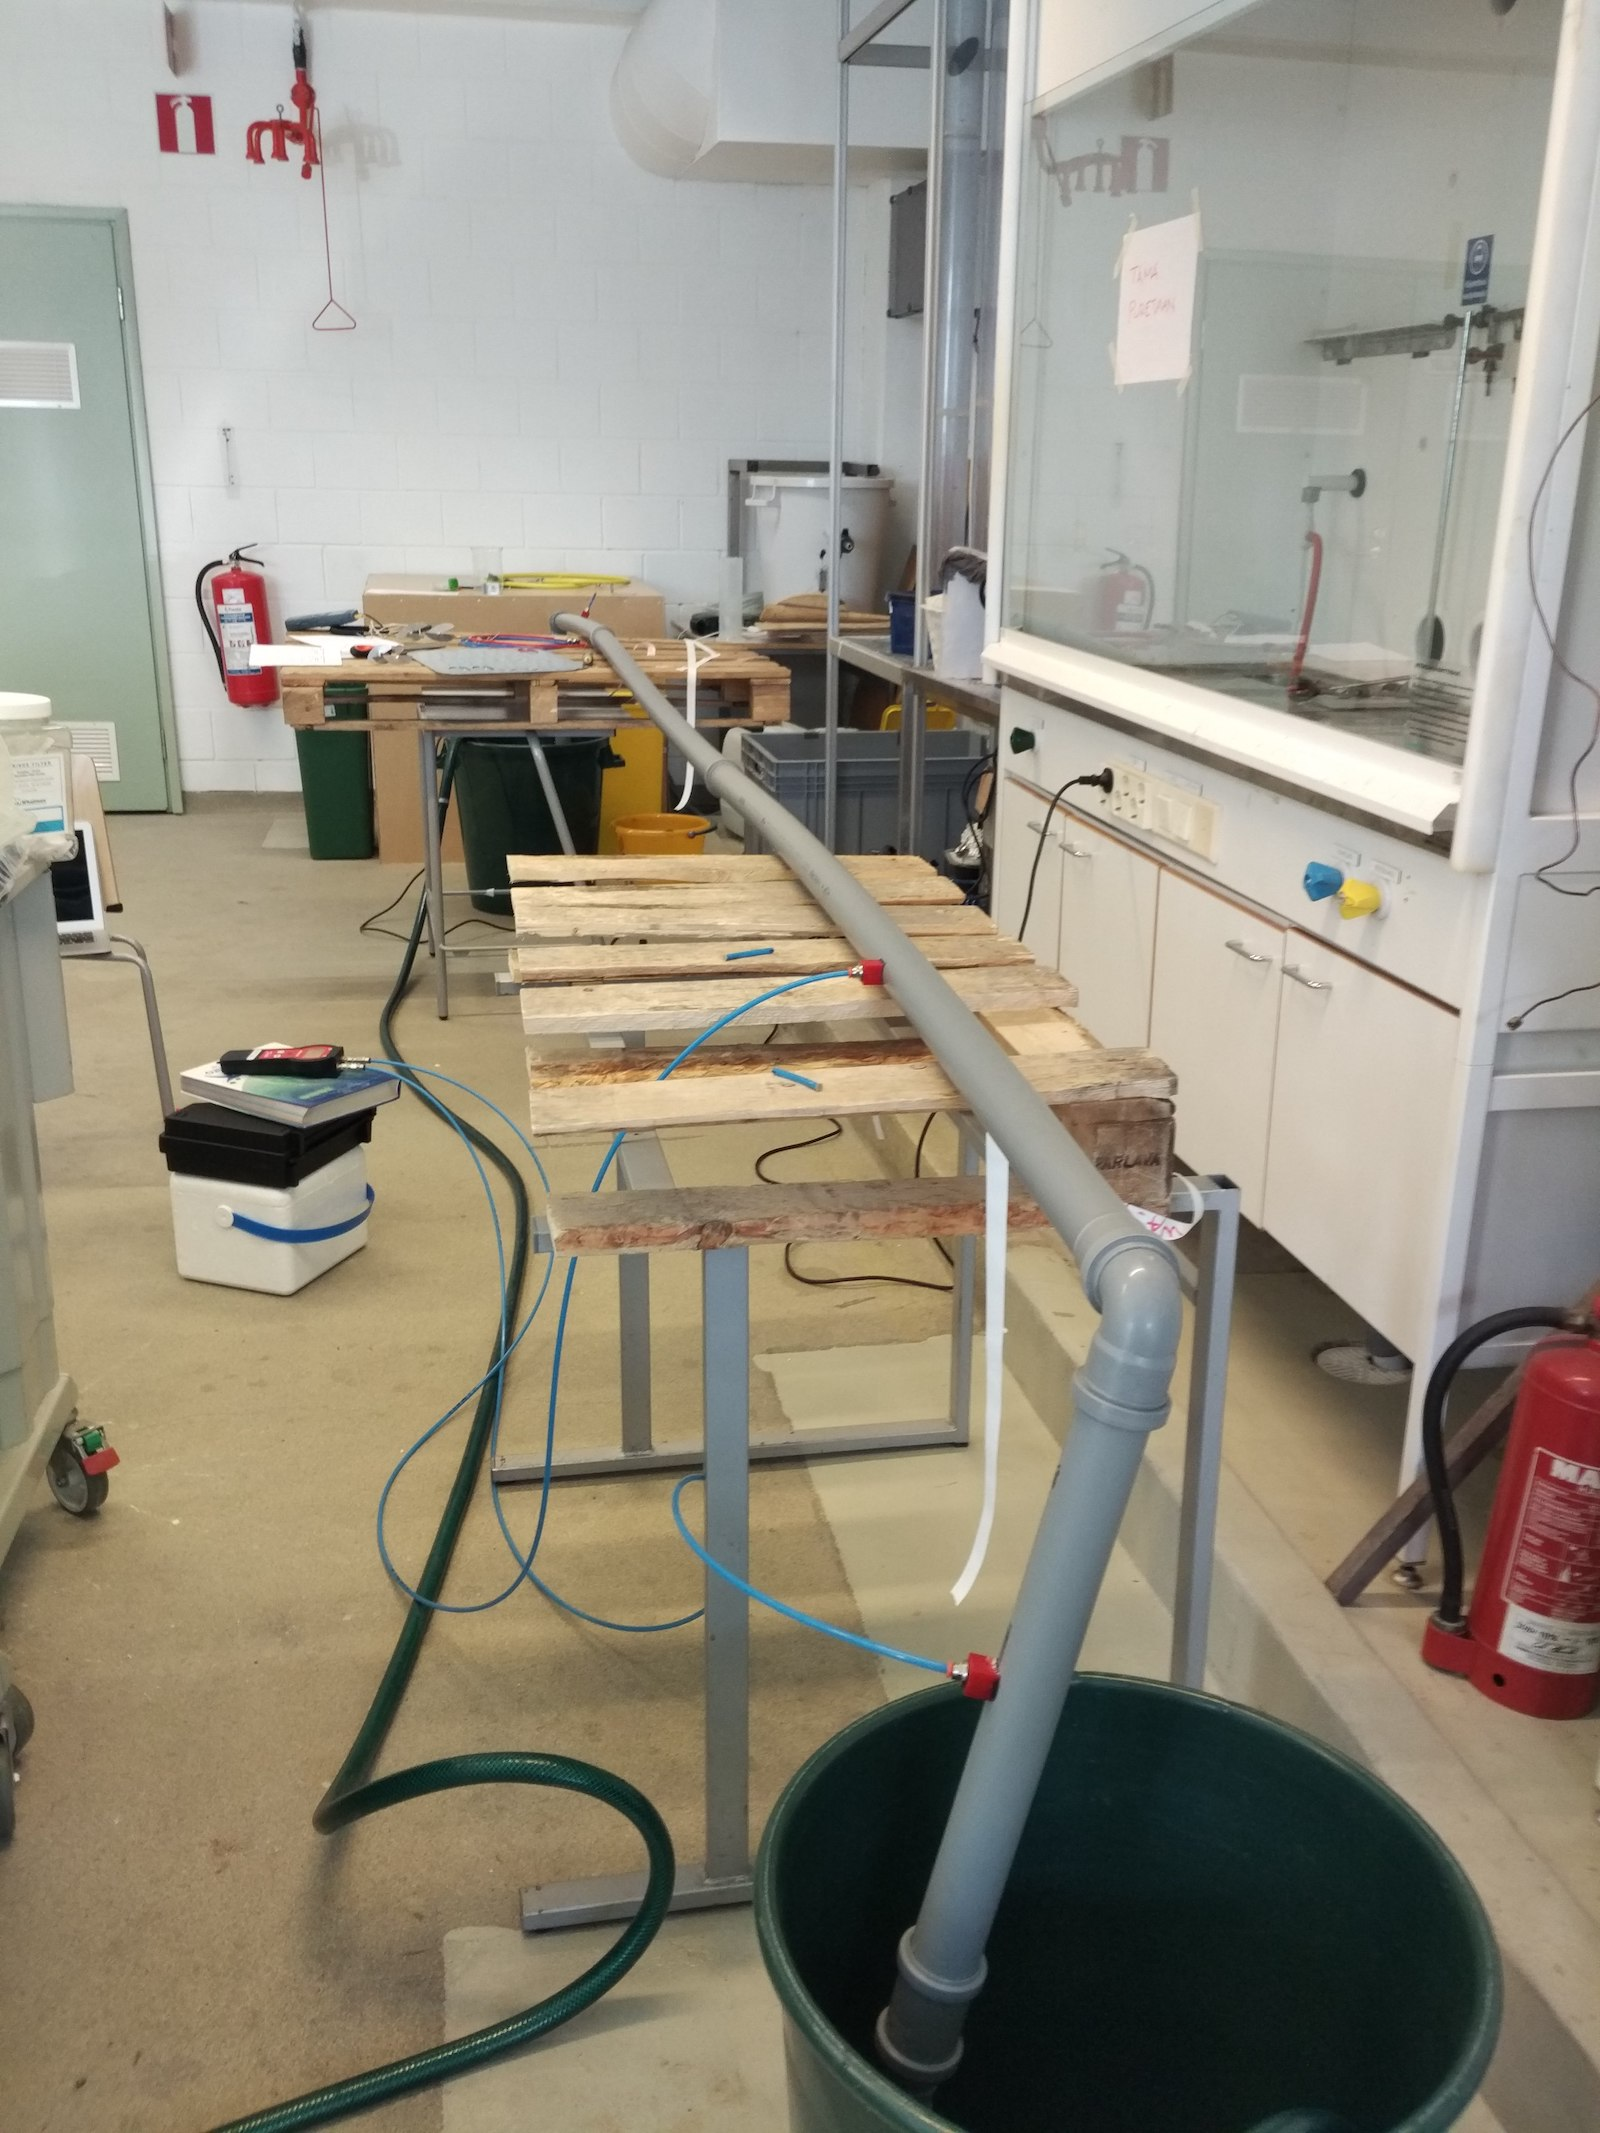
\includegraphics[width=6cm]{wholepipe}
  \caption{View of the whole test pipeline in Metropolia's lab }
  \label{fig:wholepipe}
\end{figure}
\newpage

\textbf{Connectors, pump and vessels}\newline
Plastic connectors were 3-D printed. Pressure meter’s hoses were attached to the pipe by 4 plastic connectors glued above small holes on the pipe (see figure \vref{fig:connector}). Voxers were separated from a metal sheet, bent, twisted following given instruction, and inserted into various positions of the pipeline (see figure \vref{fig:vox}). As mentioned before, the positions of Voxer were mainly at the end of each pipe. The system was set above the ground with 2 vessels at each side to keep the flow going with gravity, one as a water reservoir and one for precaution leaking. A pump was positioned in the water reservoir and connected with the starting pipe by a hose. Water was delivered through the system and come back to the water reservoir. The ending pipe was submerged completely into the water to balance the static pressure in the system (see figure \ref{fig:subpipe}). The flow direction was from right to left. 

\begin{figure}[!htb]
   \begin{minipage}{0.48\textwidth}
     \centering
     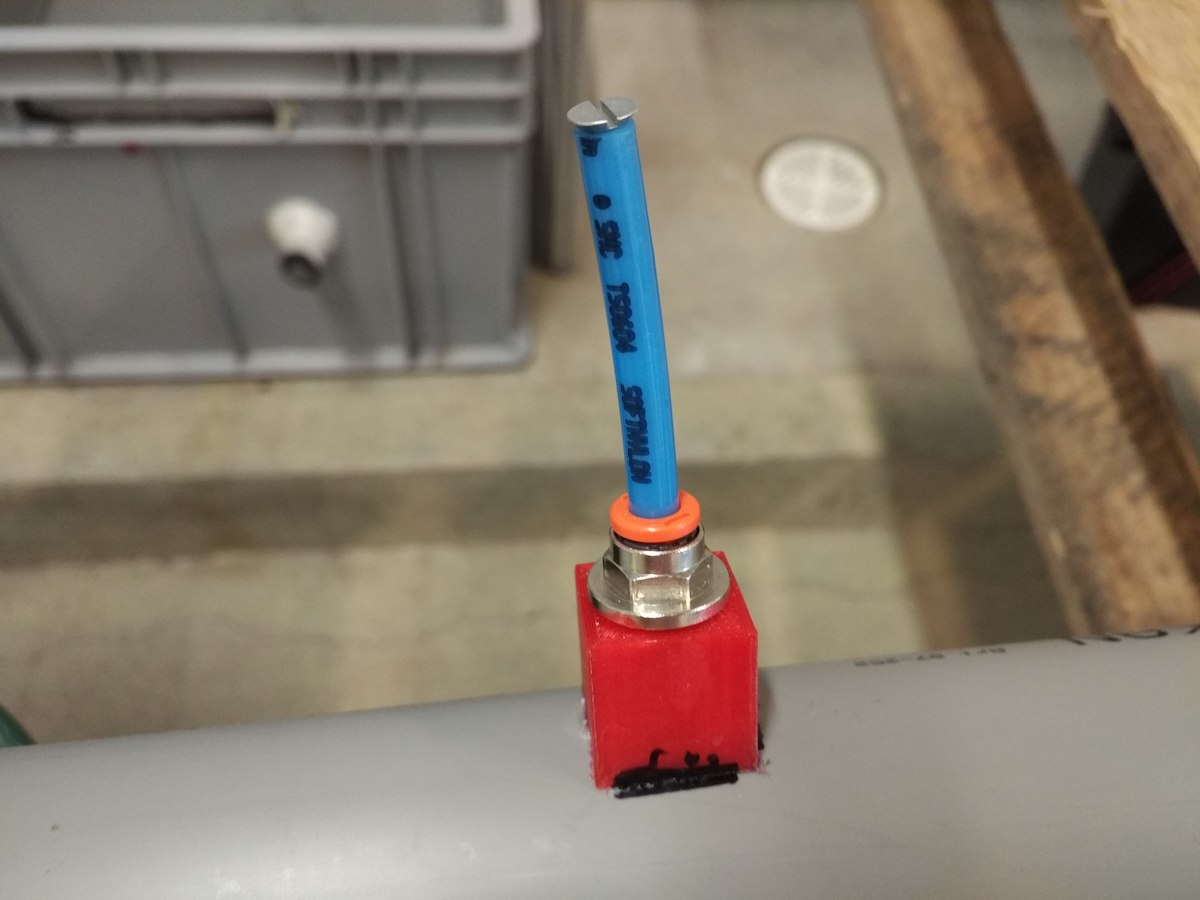
\includegraphics[width=0.9\linewidth]{connector}
     \caption{Connector as measuring points}\label{fig:connector}
   \end{minipage}\hfill
   \begin {minipage}{0.48\textwidth}
     \centering
     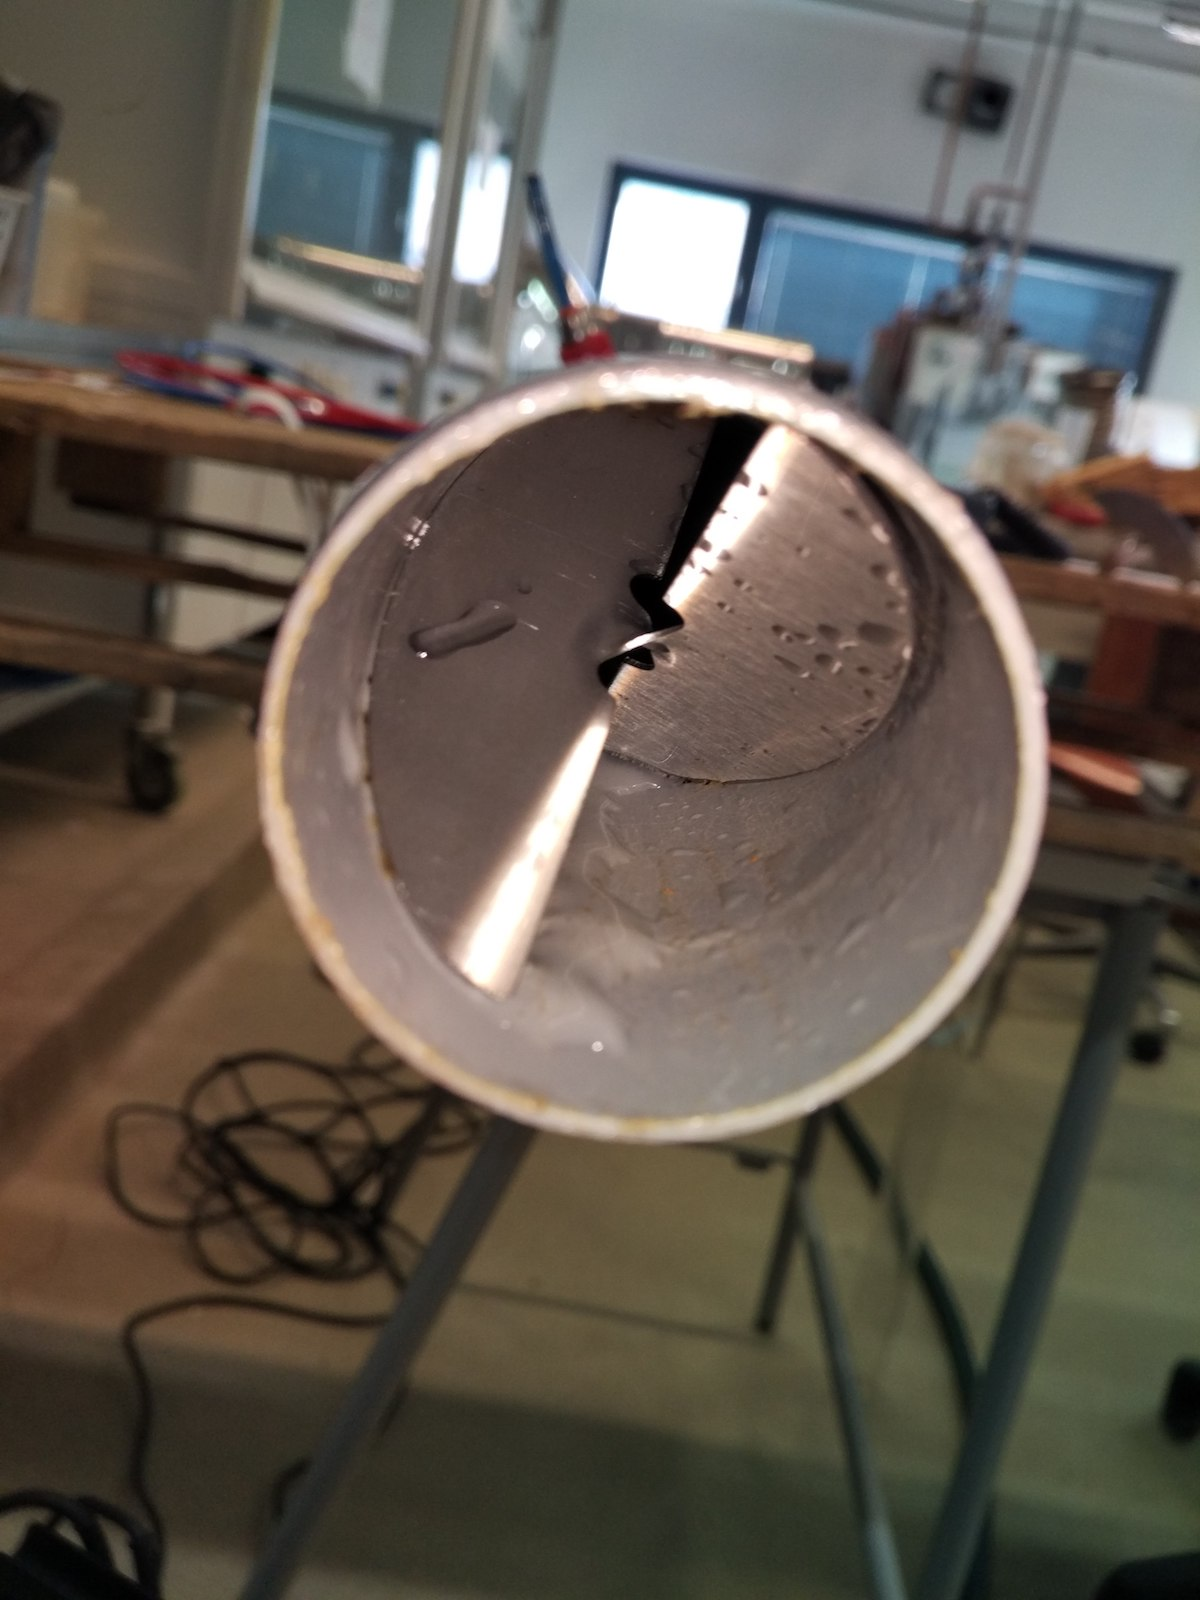
\includegraphics[width=.6\linewidth]{vox}
     \caption{Voxer wing inside pipe}\label{fig:vox}
   \end{minipage}
\end{figure}


\begin{figure}[h]
  \centering
  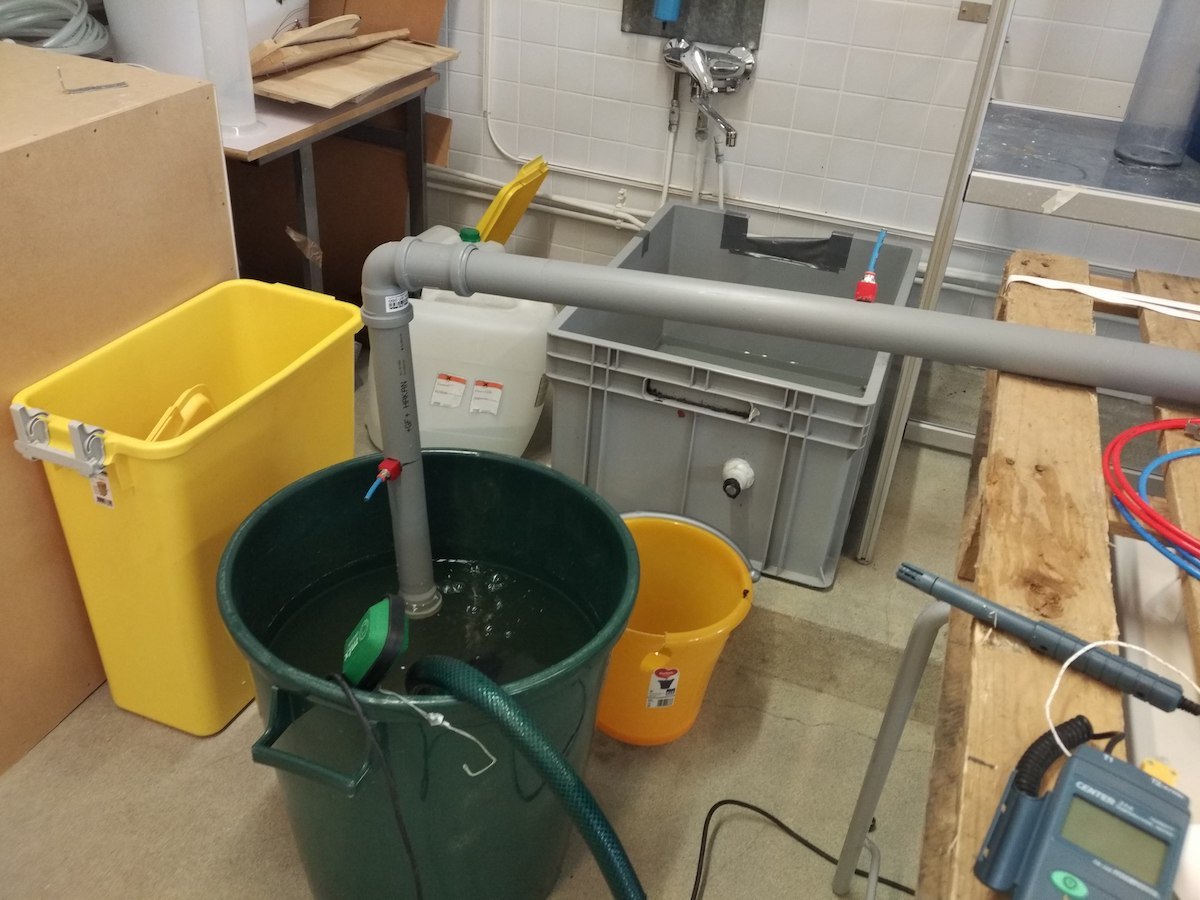
\includegraphics[width=9cm]{sub-pipe}
  \caption{ The ending pipe was submerged into water in reservoir}
  \label{fig:subpipe}
\end{figure}
\newpage

\subsection{Result and analysis}

Since the data frame acquired from lab experiment is really extensive, the values from each measurement were aggregated and demonstrated through the following graphs.

\begin{figure}[h!]
  \centering
  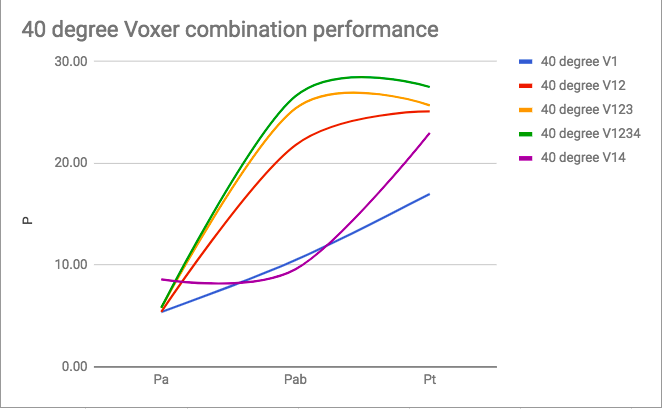
\includegraphics[width=11cm]{40d_graph}
  \caption{ Compare performance of each combination from Voxer $40^{\circ}$ DN40}
  \label{fig:40d}
\end{figure}

In figure \vref{fig:40d}, all of the combinations which have Voxer $40^{\circ}$ DN40 are compared with each other. When the flow started through the $1^{st}$ Voxer in section A, most of the pressure changes from different combinations result in the similar value around $5$ to $7$ millibars ($mb$). Section A has the $1^{st}$ Voxer before the curve. This shows that the behavior of flow after each rotation in the pipeline in section A is the same with each other. Starting from section B, we see the drastic change between $V1$, $V14$ and the rest of Voxer combinations. The pressure changes between in inflow and before section C are truly dramatic from $7\ mb$ to more than $25\ mb$ according to combinations with more than 2 Voxers in the pipeline. When comparing pressure of section A and B between combination $V1$ and $V14$, $V14$ is appeared to have less pressure drop than $V1$. From total pressure drop point of view, $V1$ has the lowest pressure change while $V14$ and the rest of combination meet around $24$ to $27\ mb$. From this graph, it can be seen that 1 Voxer at position $V1$ results in the lowest pressure change which means that the pressure loss was reduced. 
\newpage

\begin{figure}[t]
  \centering
  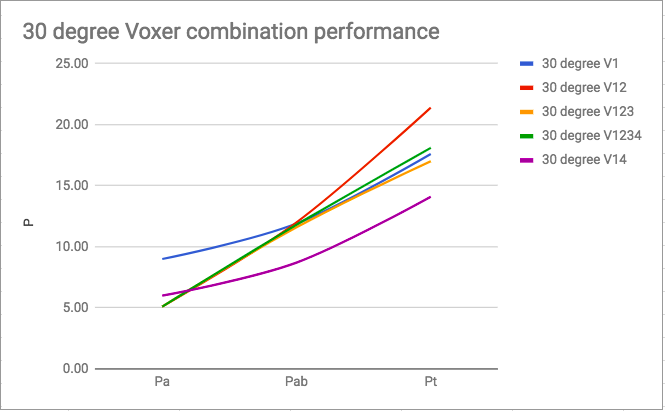
\includegraphics[width=11cm]{30d_graph}
  \caption{Compare performance of each combination from Voxer $30^{\circ}$ DN40}
  \label{fig:30d}
\end{figure}

Figure \ref{fig:30d} illustrates the operation of Voxer $30^{\circ}$ DN40 from five Voxer combinations. The trendlines from these combinations of Voxer $30^{\circ}$ are much more uniform than those trendlines of Voxer $40^{\circ}$. They all started in section A with a short range of pressure change from $5$ to $9 \ mb$. After section A and B, most of the trendlines except $V14$ meet each other at the intersection of $12\ mb$. From here, these trendlines don't separate at total pressure ($0.5$ to $1 \ mb$ difference) from each other that much except $V12$ ($22\ mb$). Meanwhile, $V14$ keeps the parallel trendlines at the lower level from $6$ to $14\ mb$.
\begin{figure}[h!]
  \centering
  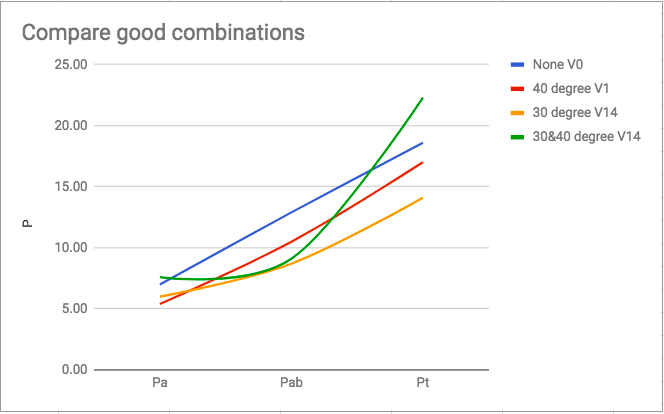
\includegraphics[width=11cm]{compare_graph}
  \caption{ Comparison among good Voxer combinations }
  \label{fig:compare}
\end{figure}

We compare the most potent combinations of each Voxer type with the mixed combination and standard pipeline with no Voxer inside in figure \vref{fig:compare}. It can be clearly seen that the correlation of pressure change along the pipe of the standard pipeline, combination $V1$ of Voxer $40^{\circ}$ and combination $V14$ of Voxer $30^{\circ}$ are almost parallel with each other. The mixed combination V1 (Voxer $30^{\circ}$ ) and V4 (Voxer $40^{\circ}$ ) actually reduces sectional pressure loss comparing to original pipe but later it leads to the increase in total pressure change when the flow goes through Voxer $40^{\circ}$  at the end of the pipe. 

\begin{figure}[h!]
  \centering
  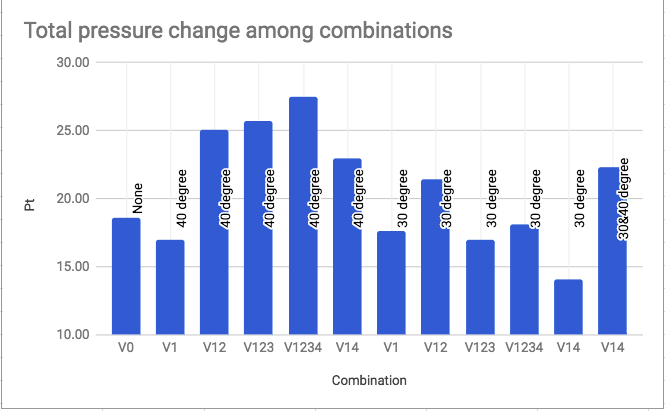
\includegraphics[width=11cm]{Pt_graph}
  \caption{ Total pressure change among all combinations}
  \label{fig:pt}
\end{figure}

Figure \vref{fig:pt} points out those combinations which diminished the flow reduction in the system. Those which reduced the little amount of pressure drop were $40^{\circ}- V1$, $30^{\circ} - V1$, $30^{\circ} - V123$ and $30^{\circ} - V1234$. It can be concluded that the largest reduction in total pressure is combination $V14$ of Voxer $30^{\circ} DN40$. In general, Voxer $30^{\circ}$ performed better than Voxer $40^{\circ}$. More Voxers in the pipeline, especially inside the main horizontal pipeline would increase pressure change of system in total.  

\section{Experimentation in Keravan Energy}

With the result of the laboratory test, we used them as the references to the design of alternative pipeline in the cooling system. Information about the system was given from Keravan Energy. It is known that the income flow rate is around $2\ l/s$ (local measure) at $1\ bar$ pressure. The input temperature is $6\celsius$  and the output temperature is $16\celsius$. 
Since it is not advised to interfere with the existing pipeline of the cooling system, we should assemble an alternative pipeline with characteristics needed for the comparative measurement. In this experiment at Keravan Energy, we observe the behavior of Voxer under realistic uncontrolled condition. The assembly was done in Metropolia's mechanical laboratory.  

\subsection{Experiment's design}

From the observation of original pipeline section (see figure \vref{fig:original_pipe}, it is clear that Voxer couldn't be placed inside rubber hoses but inside straight steel circular pipe. This also applied to positions of measuring points to measure inflow before the curve and outflow after the pipe bend. The water flow rate in Keravan Energy is much higher than the one from the pump used in the lab test. So there are chances that water would be leaked from the pipe leading to more energy loss. The fact that Voxer wing should be easy to remove from the pipe between different combinations  is taken into consideration.

\begin{figure}[h]
  \centering
  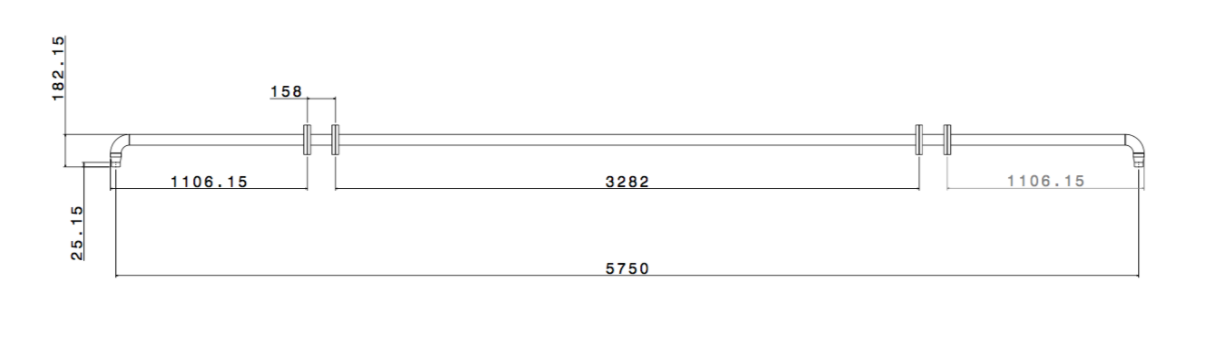
\includegraphics[width=14cm]{cadkerava}
  \caption{ Drawing of pipeline for experiment at Keravan Energy}
  \label{fig:cadkerava}
\end{figure}

A design of pipeline shown in figure \vref{fig:cadkerava} is the experiment's solution for most of the problems above. The length of pipeline section was taken from \gls{cad} documentation of Keravan Energy and measured again at the site. In this setup, there were maximum 2 Voxers tested in the pipeline. Voxer wings were placed from the separated pipes (we call them Voxer pipes) with flanges which would be easily connected to the main pipe. 
Rubber hoses were attached to the pipeline by reducers at each side. The measuring points were positioned on the reducers to catch inflow and outflow pressure as well as the middle of the long pipe. We divided this testing pipeline into 2 sections. Section A is from inflow reducer to middle point of the pipe. Section B is from the middle point to the outflow reducer. The same principles were applied to pressure changes of this pipeline: 
\begin{align}
\Delta P_t&= P_ab = P_a + P_b
\end{align}
In this experiment, $\Delta P_{ab}$ is the total pressure change in pipeline; $P_a$ and $P_b$ are  ther pessure change in section A and section B.
There were two types of Voxer were also tested (Voxer $30^{\circ}$ DN50 and Voxer $40^{\circ}$ DN50). The first Voxer was positioned in section A and the second one was in the other section. The measurements of the $2^{nd}$ sectional and total pressure were measured by pressure meter. Three combinations of Voxer were measured: None (indicating empty pipe with no Voxer inside), degree 30 (2 Voxers $30^{\circ}$ DN50), degree 40 (2 Voxers $40^{\circ}$ DN50) (see table \ref{table:kerava}). The material of pipes is \gls{cs}. All of the components were purchased from Ahnsell and assembled in Metropolia's mechanical lab.

\begin{table}[h]
  \centering
  \caption{Voxer combinations in Keravan Energy's test}
  \begin{tabular}{l*{2}{c}}
Type             & V0 & V12 \\
\hline
None & X & -   \\
30 degree           & - & X   \\
40 degree          & - & X   \\
\end{tabular}
  \label{table:kerava}
\end{table}

\subsection{Setting of experiments}

\subsubsection{Components Assembly}

\textit{Measuring points}\newline
A metal rod was cut into parts and tapped to create a thread for measuring point connectors. Then holes were drilled to create contact spaces with the pressure meter. The cylinder metal parts were welded into reducers and the middle point of long pipe above those holes. Figure \vref{fig:coke} presents the final look of measuring points.

\textit{Pipes}\newline
The main $6\ m$ carbon steel pipe was cut into parts: two Voxer pipes, two side pipes, and one long middle pipe. Voxer pipes and long middle pipe were welded with two flanges on each side. Then curves were welded together with side pipes and reducers as a unit. Before welding, the reducers were shaped to fit with the rubber hoses (see figure \vref{fig:sidepipe}).

\begin{figure}[!htb]
   \begin{minipage}{0.48\textwidth}
     \centering
     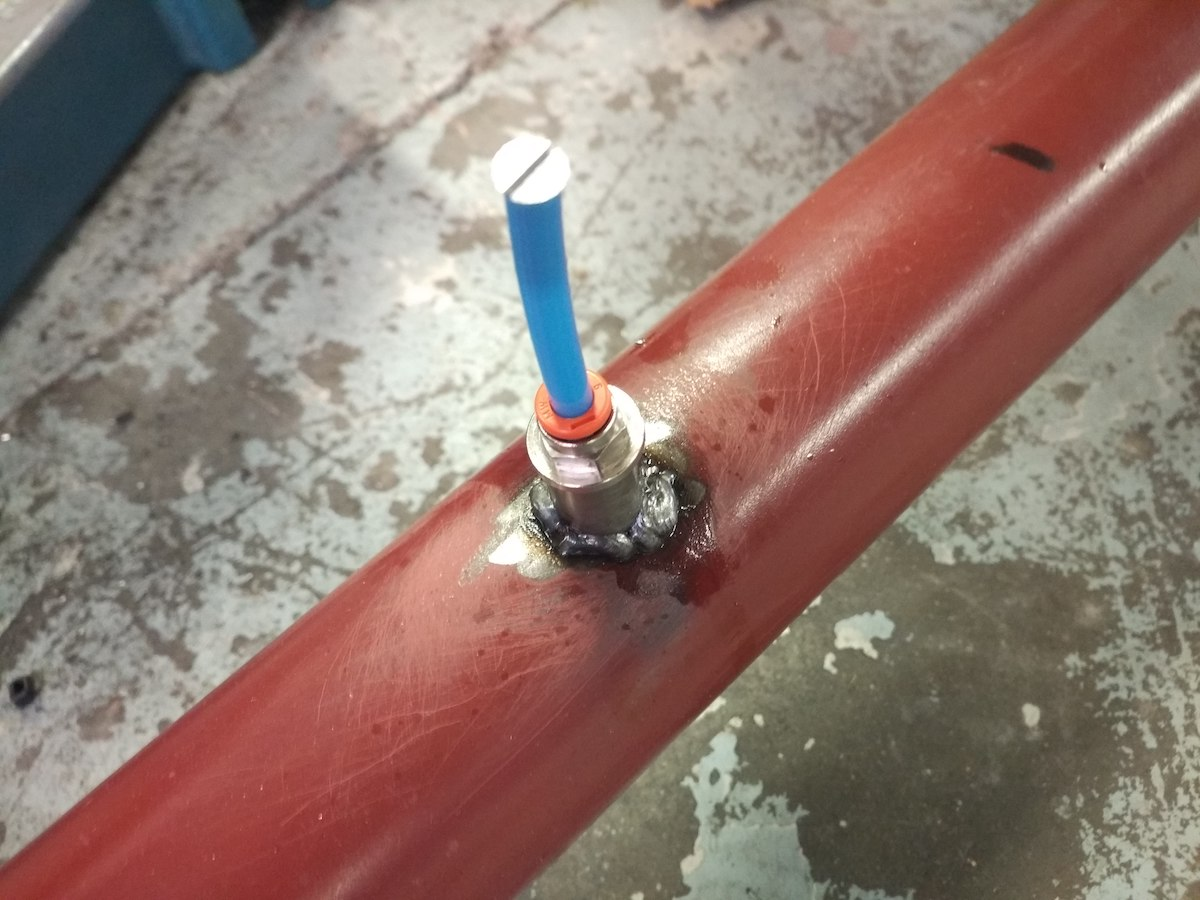
\includegraphics[width=0.8\linewidth]{connect_ke}
     \caption{Metal connector as measuring points}\label{fig:coke}
   \end{minipage}\hfill
   \begin {minipage}{0.48\textwidth}
     \centering
     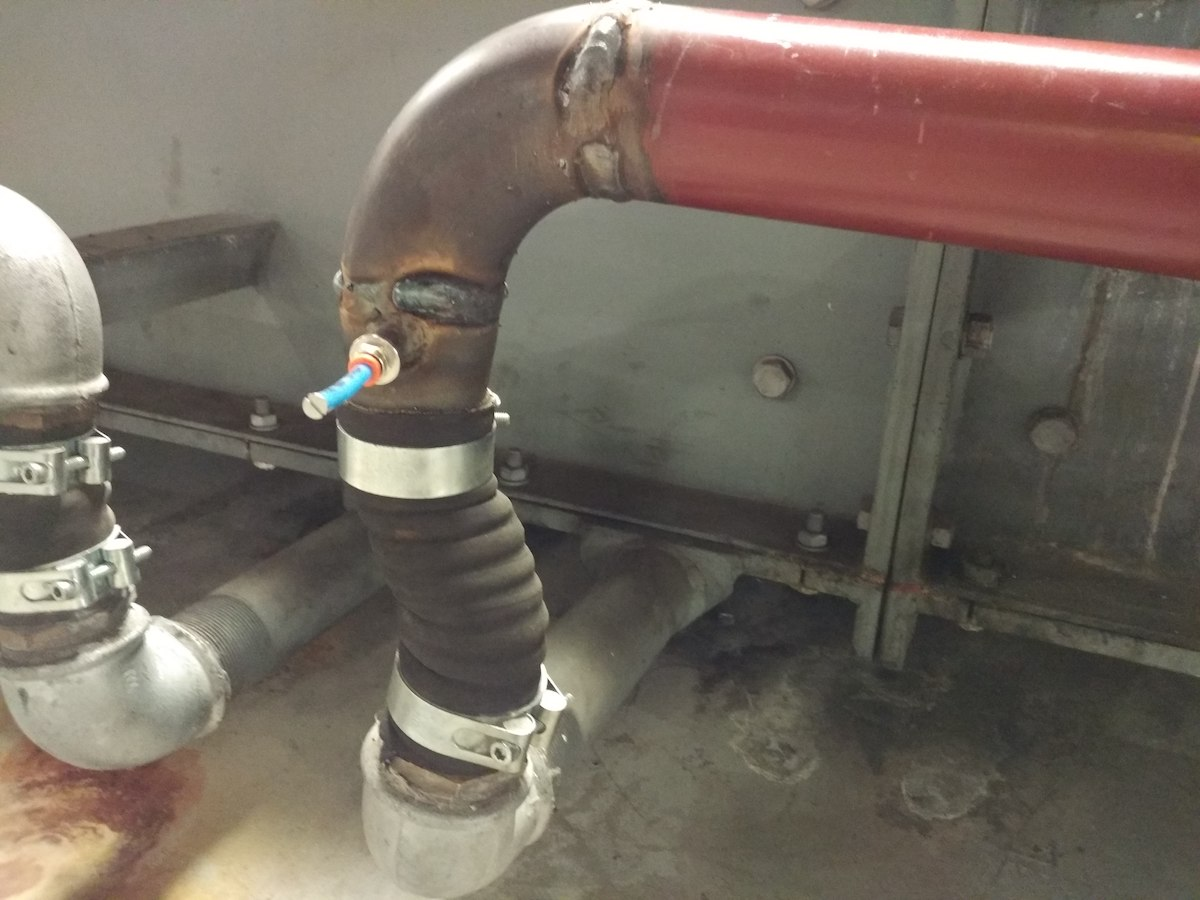
\includegraphics[width=.8\linewidth]{new_side_pipe}
     \caption{Curve, reducer and side pipe}\label{fig:sidepipe}
   \end{minipage}
\end{figure}

\subsubsection{Setting up in Keravan Energy}

At Keravan Energy, the original pipeline section was removed and altered with our testing pipeline. The frame was raised to hold the weight of the new pipeline with higher height than the original one. New rubber hoses were cut to fit the new pipeline. After testing and adjusting some minor problems in the system, the flow rate was adjusted from $2$ to $0.8\ l/s$ to reduce the pressure applied to minor leaking points along the pipe. Figure \vref{fig:overview} shows an overview of the setting.

\begin{figure}[h]
  \centering
  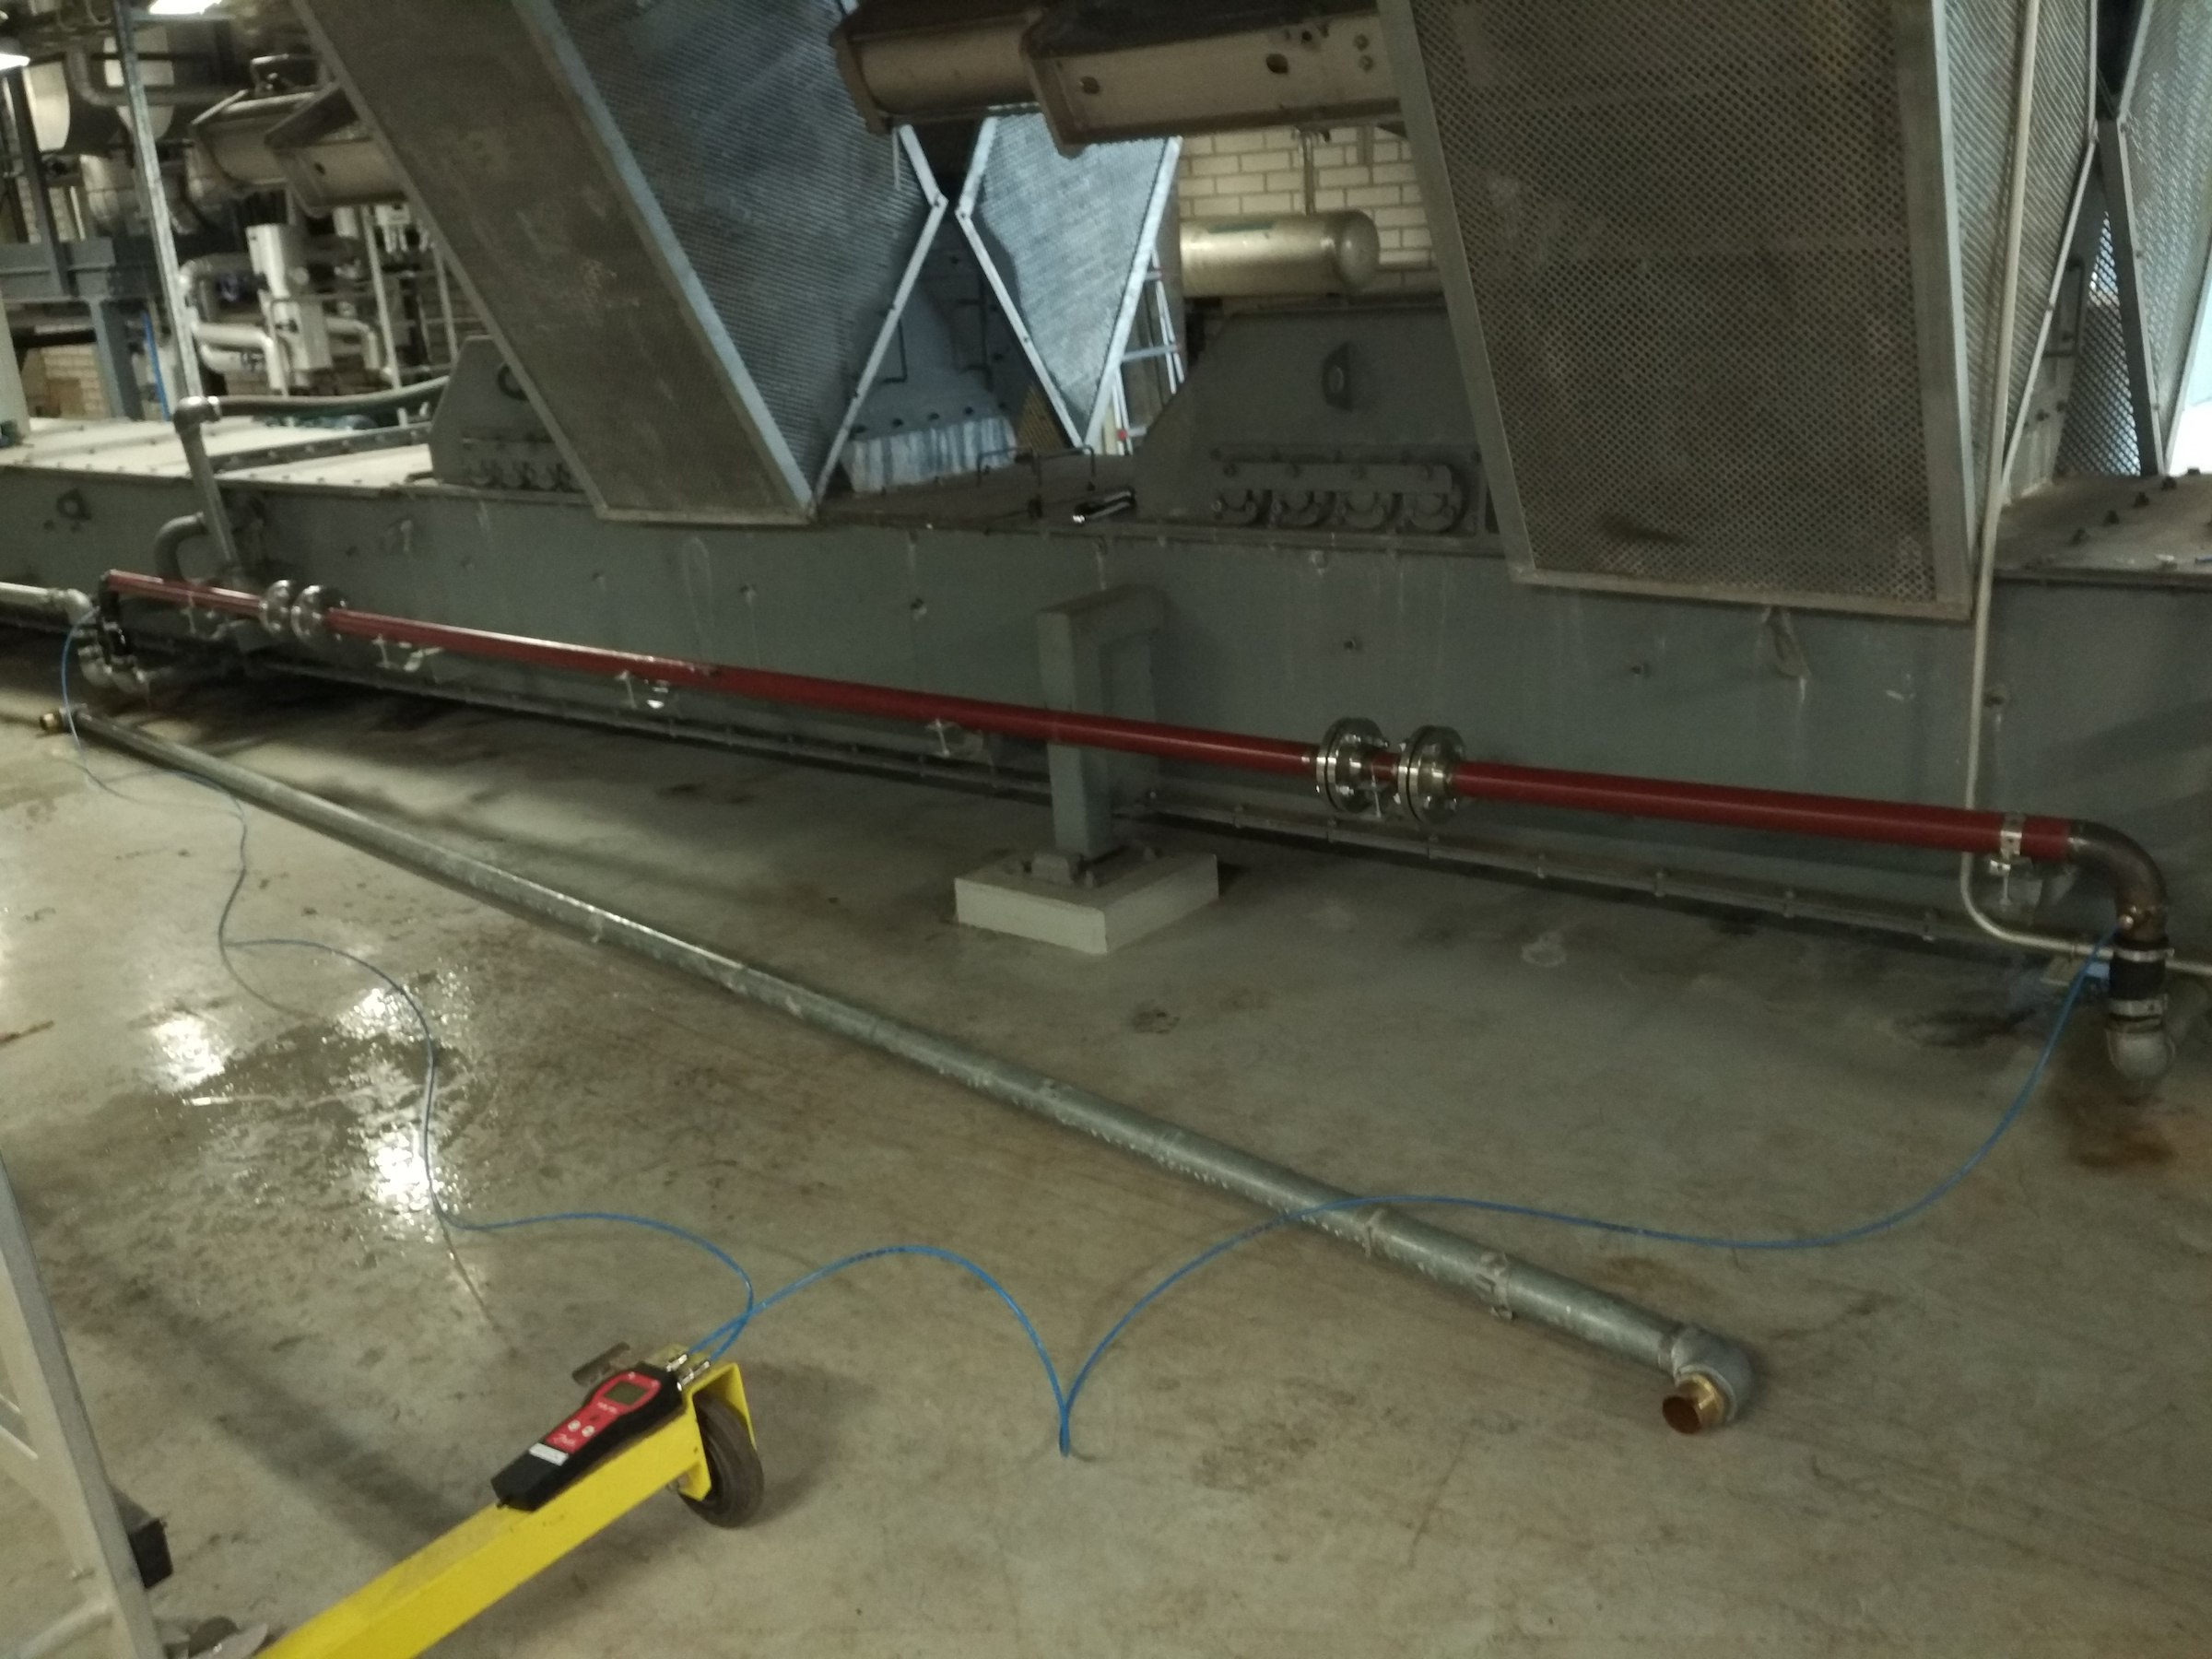
\includegraphics[width=10cm]{overview_test}
  \caption{ An overview of the testing pipeline}
  \label{fig:overview}
\end{figure}

\subsection{Result and analysis}

From the observations through the pressure meter, the pressure values of each measurement were not stable and varying in a large range. Apparently with an unfitted framework, the system didn't get really good support so the pipeline resonated axially and radically. The result from Kervan Energy experiment was not as definate as the result of lab experiment since the measurement was performed under an uncontrolled condition in such limited amount of time. Therefore each measurement was recorded in separated videos and transcribed into separate \gls{csv} files. In the experiment, $P_{\text{b}}$ and $P_{\text{ab}}$ were recorded. There are 100 points from each measurement transcribed. The flow rate of the system was maintained around $0.8\ l/s$ throughout the whole experiment. There were some minor water leakages around measuring points as well. All of these factors led to pressure value scattering and a significant uncertainty in the result.

\begin{figure}[h]
  \centering
  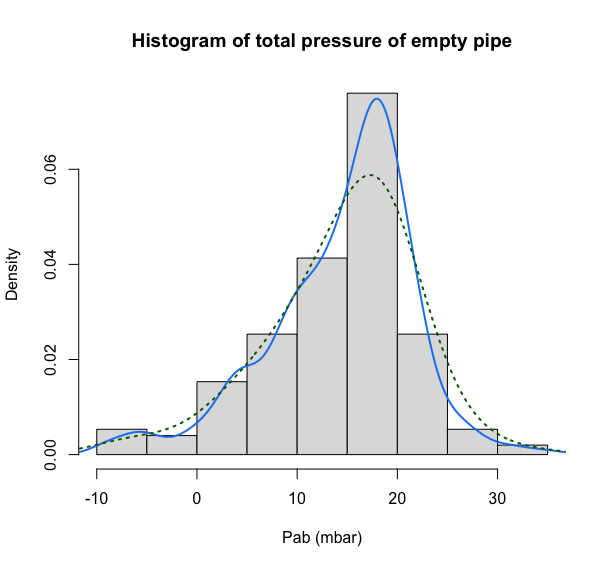
\includegraphics[width=9cm]{hist_none}
  \caption{ Histogram of total pressure change values in empty pipeline}
  \label{fig:histnone}
\end{figure}

From Figure \ref{fig:histnone}, it can be seen that the total pressure inside the empty piping section varies in a large range from $-10$ to $30\ mb$. The negative values can be explained as the possibility of \gls{cavit} occurrence due to high velocity. The most occurring pressure values are ranged from $10$ to $20\ mb$. The dotted line illustrated smoothened density line of the total pressure in the empty pipe. 

\begin{figure}[h]
  \centering
  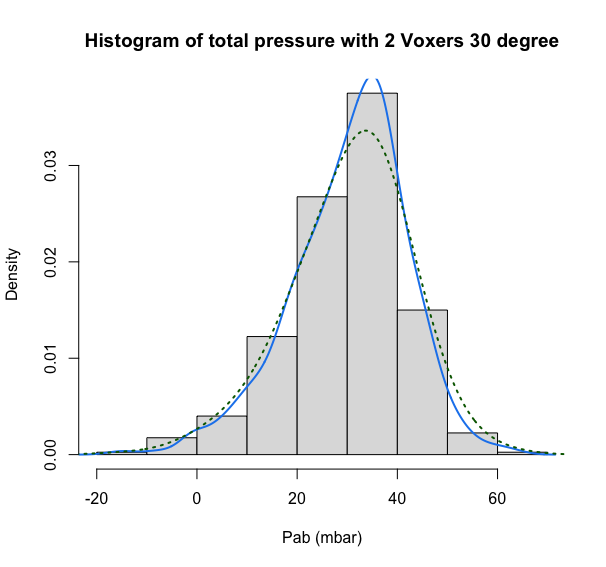
\includegraphics[width=9cm]{Hist_30d}
  \caption{ Histogram of total pressure change values with Voxer $30^{\circ}$}
  \label{fig:hist30d}
\end{figure}

It is illustrated in figure \ref{fig:hist30d}, the total pressure of a combination of two Voxers $30^{\circ}$. Values range vastly from $0$ to $50\ mb$. The most popular values in this combination vary from $20$ to $40\ mb$.

\begin{figure}[h]
  \centering
  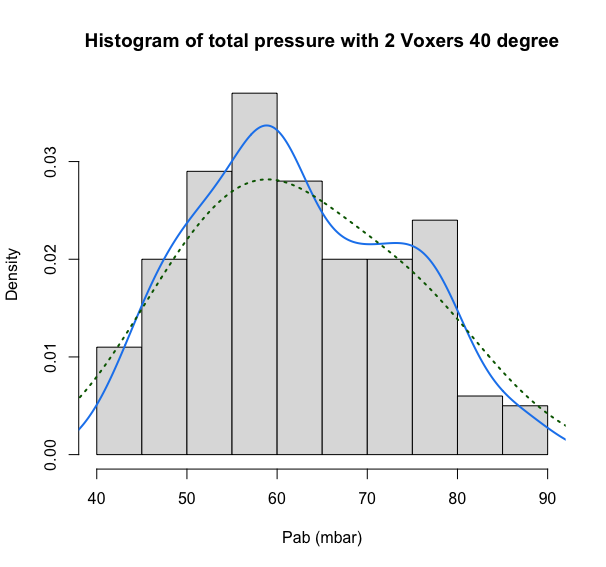
\includegraphics[width=8cm]{Hist_40d}
  \caption{ Histogram of total pressure change values  with Voxer $40^{\circ}$}
  \label{fig:hist40d}
\end{figure}

There are some differences in combination Voxer $40^{\circ}$ with empty pipe and Voxer $30^{\circ}$ shown in figure \ref{fig:hist40d}. The distribution of two other graphs shows the pattern of normal distribution while this graph shows a large range of value distribution. Values vary from $40$ to $90\ mb$, which is much higher than measurements from the empty pipe and Voxer $30^{\circ}$. Pressure change values occur most around $50$ to $65\ mb$ and from $75$ to $80\ mb$.

\begin{figure}[h]
  \centering
  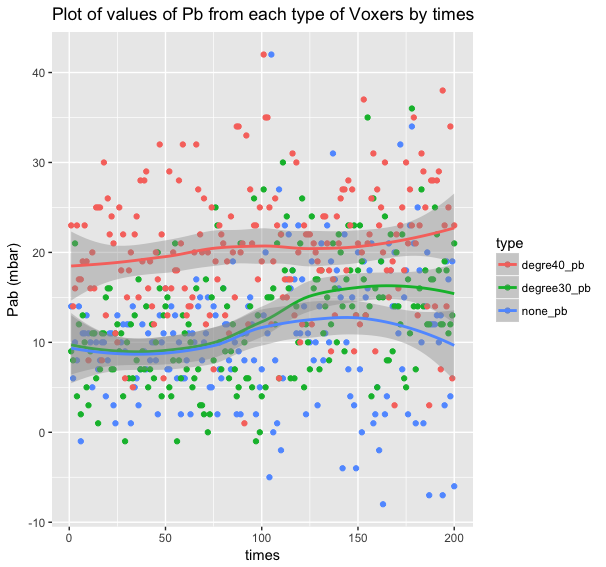
\includegraphics[width=9.5cm]{Pb_plot}
  \caption{ Graph of $P_{\text{b}}$ among three combinations throughout time}
  \label{fig:pbplot}
\end{figure}

Each point in figure \vref{fig:pbplot} represents pressure value of section B with $2^{nd}$ Voxer in the piping section throughout recorded times. The line smoothens the trend of pressure values in each type of combination. From here, we can see that trendline of Voxer $40^{\circ}$ is quite constant with pressure changes from $17$ to $21\ mb$. Meanwhile, the pressure change's trendlines of empty pipe and Voxer $30^{\circ}$ are also aligned with each other. 

\begin{figure}[h]
  \centering
  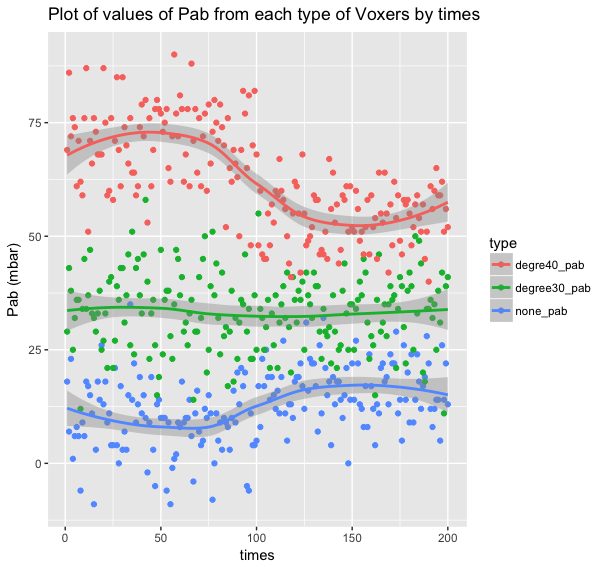
\includegraphics[width=9.5cm]{Pab_plot}
  \caption{ Graph of $P_{\text{ab}}$ among three combinations throughout time}
  \label{fig:pabplot}
\end{figure}

Figure \ref{fig:pabplot} shows the significant division of value range among 3 combinations at total pressure change. Voxer $40^{\circ}$  has the largest pressure drop range and reducing pressure drop trendline over time. Empty pipe and Voxer $30^{\circ}$ have stable pressure drop over time. Total pressure drop range of Voxer $30^{\circ}$ is $20\ mb$ larger than the empty pipe. 
\newpage

\begin{figure}[h]
  \centering
  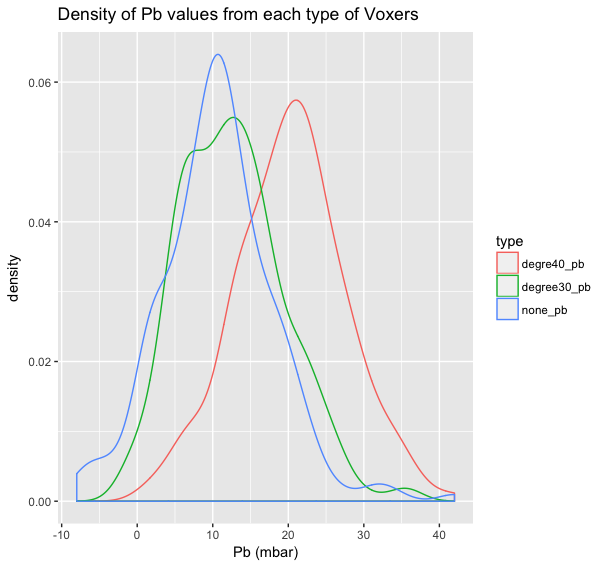
\includegraphics[width=9cm]{Pb_density}
  \caption{ Comparison $P_{\text{b}}$ values density among three combinations}
  \label{fig:pbdensity}
\end{figure}

In the technical document, Mr. Pylkkänen mentioned that the optimal position to place the Voxer is where turbulence occurs and flow losses normally. This might be a technically correct statement in section B, where $2^{nd}$ Voxer was placed before the last curve. In figure \ref{fig:pbdensity}, we see the density of pressure change in section B among 3 combinations. Except for Voxer $40^{\circ}$ combination, Voxer $30^{\circ}$ presents that it has the potential to reduce pressure drop when compared with empty pipe since it overlaps with the distribution line of empty line with a lower probability.  

\begin{figure}[h]
  \centering
  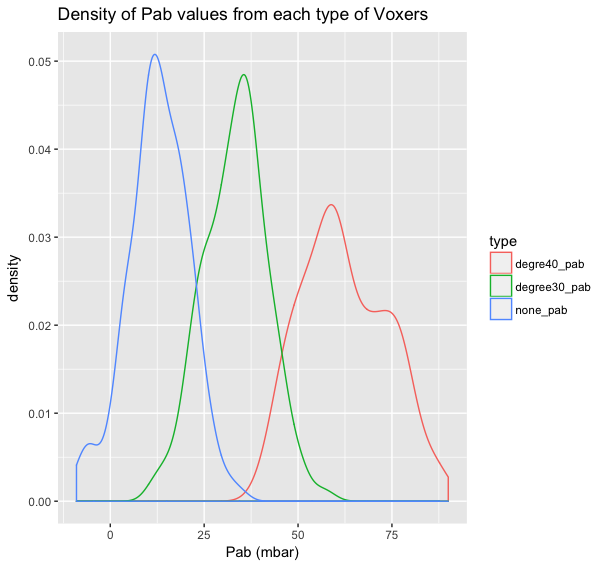
\includegraphics[width=9cm]{Pab_density}
  \caption{ Comparison $P_{\text{ab}}$ values density among three combinations}
  \label{fig:pabdensity}
\end{figure}

In the whole pipeline section presented in figure \ref{fig:pabdensity}, the distribution line of each combination distinctly separates from each other. The distribution line with lowest pressure value is empty, following by Voxer $30^{\circ}$ and Voxer $40^{\circ}$  is the highest.
\clearpage %force the next chapter to start on a new page. Keep that as the last line of your chapter!
